\chapter{Literature Review} \label{sec:litrev}

This chapter reviews the literature related to DFL for ND problems, and introduces the mathematical notions used in later sections with a common notation. We split this review into four sections. Section~\ref{sec:litrev:network-design} covers the literature on ND, which are combinatorial optimization problems that compute the best network structure in a graph to fulfill demand between origin and destination points. Section~\ref{sec:litrev:dfl} explores different approaches to DFL. Originating at the intersection of ML and operations research, DFL attempts to integrate a data-decisions pipeline's prediction and optimization steps. Section~\ref{sec:litrev:inverse-optimization} focuses on IO, a field of mathematical optimization which consists of recovering model parameters given optimal solutions to the model. Finally, Section~\ref{sec:litrev:discussion} concludes by discussing directions for our research project and current gaps in the literature.

%%%%%%%%%%%%%%%%%%%%
\section{Network Design} \label{sec:litrev:network-design}
%%%%%%%%%%%%%%%%%%%%

Many problems in operations research, particularly in transportation and logistics, can be expressed as ND problems. The literature related to ND is extensive \citep{hirschFixedChargeProblem1968, gomoryMultiTerminalNetworkFlows1961, gendronMulticommodityCapacitatedNetwork1999a, cadarsoStrategicMultistageOperational2018}, and a comprehensive review is out of the scope of this thesis. We base our review of ND on the book from \cite{crainicNetworkDesignApplications2021}. It offers a recent and extensive survey of ND, including its applications to transportation problems. They first present general formulations for ND problems and exact and approximate methods for solving them. They then explore specific applications of ND to transportation and logistics. We use the book's path-based formulation for the deterministic Multi-Commodity Fixed-Charge Network Design problem (MCFND). The authors showcase linear relaxations of the MCFND problem and valid inequalities that can lead to stronger bounds. The stochastic variant of the MCFND is also explored, in which design and flow costs, arc capacities, and commodity demands are not known exactly, but all follow a random distribution. The authors formulate the problem as a two-stage stochastic program and then briefly explore solving such programs using Sample Average Approximation (SAA). The book mainly explores the optimization side of a ND data-decisions pipeline, with less attention paid to stochastic variants and estimation of problem parameters. 

We formulate the MCFND here as in \cite{crainicNetworkDesignApplications2021}. The MCFND is defined on a graph $\mathcal{G} = (\mathcal{N}, \mathcal{A})$ comprised of nodes $\mathcal{N}$ and arcs $\mathcal{A}$ connecting them. The formulation includes a set of commodities $\mathcal{K}$, each with an origin and destination node $\{(\mathrm{orig}(k), \mathrm{dest}(k)) : k \in \mathcal{K}\}$. Each commodity $k$ has a demand $d^k$ that the network must fulfill. At every node $n \in \mathcal{N}$, $d_n^k$ specifies the demand for commodity $\commodities$ as follows:
\begin{equation}
d_n^k = \begin{cases}
    -d^k, & n = \mathrm{orig}(k),\\
    d^k, & n = \mathrm{dest}(k),\\
    0, & \textrm{otherwise}.
\end{cases}
\end{equation}
Each arc $(i, j)\in \mathcal{A}$ has a capacity $u_{ij}$. It costs $f_{ij}$ to build arc $(i,j)$ and $c^k_{ij}$ for commodity $k$ to flow across it. Binary design variables $y_{ij} \in \{0, 1\}$ indicate if arc $\arcs$ is built, and flow variables $\xijk \geq 0$ indicate the quantity of commodity $\commodities$ flowing across arc $\arcs$. We obtain the following formulation for the MCFND:\\
\begin{minie}
    {\bm{x}, \bm{y}}
    {\sum_\arcs f_{ij} y_{ij} + \sum_\commodities \sum_\arcs c_{ij}^k \xijk \label{eq:litrev:mcfnd-objective}}
    {(MCFND) \label{eq:litrev:mcfnd}}
    {{}}
    \addConstraint{\sum_{j\in \mathcal{N}_i^+} \xijk - \sum_{j \in \mathcal{N}_i^-} x_{ji}^k}{= d_i^k, \quad \label{eq:litrev:mcfnd-flow-cons}}{\forall \nodes, \commodities}
    \addConstraint{\sum_\commodities \xijk}{\leq u_{ij} y_{ij}, \quad}{\forall \arcs}
    \addConstraint{\xijk}{\geq 0, \quad}{\forall \arcs, \commodities}
    \addConstraint{y_{ij}}{\in \{0, 1\}, \quad \label{eq:litrev:mcfnd-integrality}}{\forall \arcs.}
\end{minie}

\begin{defin}[Shorthand notation for MCFND] The ND problem from (\ref{eq:litrev:mcfnd}) with demands $\db$ returning optimal decision variables $x^*(\db), y^*(\db)$ is written in a shorter form:
\begin{equation*}
    (x^*(\db), y^*(\db)) = \mathrm{MCFND}(\db).
\end{equation*}
\end{defin}

When predicting the uncertain parameters of the MCFND, choosing the correct point prediction for commodity demand is just as important, if not more important, than the overall accuracy of the demand prediction.
\cite{laagePeriodicFreightDemand2022} demonstrate the benefits of greater integration between the demand prediction step and the downstream optimization problem. 
The authors address the Periodic Demand Estimation (PDE) problem for cyclic Service Network Design: a time horizon is divided into multiple periods and demand is predicted for each period over the time horizon. The multiple demand predictions are mapped to a single \textit{periodic demand}, traditionally the average of the predictions, but in this case it could be the mean, the median, the third quartile, or the maximum. 
Given this periodic demand, the system solves a multi-level optimization problem that minimizes the total design and flow costs for a cyclic service network. 
The top level designs a service network that fulfils the periodic demand. The network structure is repeated for each period in the time horizon. 
The lower level then uses the designed network and adjusts the flows to fulfill the actual demand for that period, using recourse actions. The overall PDE problem aims to find, for each commodity, the mapping that minimizes the total cost of the bilevel problem. 
Allowing the PDE problem to choose from several types of mappings, i.e., reweighting the final demand forecasts, can significantly improve the overall problem cost on real-world large-scale Service Network Design problems. Although this study does not directly use DFL, it highlights the importance of integrating the prediction and optimization steps when solving large-scale ND problems.

We have covered ND problems and their stochastic and deterministic formulations. We discussed the importance of choosing the correct point prediction when predicting uncertain ND problem parameters. In the next section, we discuss how to train prediction models to make predictions that minimize the cost in the optimization step. 

%%%%%%%%%%%%%%%%%%%%
\section{Decision-Focused Learning} \label{sec:litrev:dfl}
%%%%%%%%%%%%%%%%%%%%

In mathematical optimization problems, the model's parameters are not always known in advance and must be estimated from noisy data. This parameter prediction step is traditionally done using ML \citep{bishopPatternRecognitionMachine2006} or time series forecasting \citep{degooijer25YearsTime2006} ahead of the optimization problem. Estimating these parameters separately from the downstream optimization problem, such as with an ML model minimizing a measure of prediction error, can lead to sub-optimal decisions in the optimization problem. The development of integrated prediction and optimization techniques aims to resolve this mismatch. In this thesis, we call such integrated techniques DFL. We first review traditional prediction methods from ML and introduce a common notation for learning models in our project. We then cover DFL methods using a unified notation.

We follow textbook \cite{bishopPatternRecognitionMachine2006}, which uses ML to perform supervised regression tasks. This is the the prediction step in our project. Regression ML models make predictions about the value of a continuous random variable $\db$, given input features $\phib$ that are assumed to occur jointly with $\db$ under an unknown distribution $(\phib, \db) \sim \mathcal{D}$.
\begin{defin}[Supervised ML model]
    \label{defin:litrev:mlmodel}
    A supervised ML model $f_\theta$ defined by model weights $\theta$, takes input features $\phib$ and outputs a prediction $\dhat$ for the target variable $\db$:
    $$\dhat = f_\theta(\phib).$$
\end{defin}

Supervised ML models undergo a training phase to produce accurate predictions. Prediction accuracy is measured using a loss function $\mathcal{L}$ that compares the prediction $\dhat$ to the actual value $\db$. The most common loss functions are Mean Squared Error (MSE) and Mean Absolute Error (MAE). 
\begin{defin}[Mean Squared Error loss]
    $\mathcal{L}_{\text{MSE}}(\dhat, \db) = \lVert \dhat - \db\rVert_2$.
\end{defin}
\begin{defin}[Mean Absolute Error loss]
    $\mathcal{L}_{\text{MAE}}(\dhat, \db) = \lVert \dhat - \db\rVert_1$.
\end{defin}
Given a training dataset of $N$ independent observations $\mathcal{D}_{\text{train}} = \{(\phib_i, \db_i)\}_{i=1}^N$, the model updates its weights $\theta$ to minimize prediction the prediction loss over the training dataset. If the model is convex and differentiable with respect to the model weights, this can be done iteratively using Gradient Descent, detailed in Algorithm \ref{alg:litrev:gradient-descent}.

\begin{algorithm}
    \caption{Gradient Descent algorithm}\label{alg:litrev:gradient-descent}
    \SetKwData{Left}{left}\SetKwData{This}{this}\SetKwData{Up}{up}
    \SetKwFunction{Union}{Union}\SetKwFunction{FindCompress}{FindCompress}
    \SetKwInOut{Input}{Input}\SetKwInOut{Output}{Output}
    
    \Input{\,loss function $\mathcal{L}$ \\        
  \,learning rate $\gamma \geq 0$ \\%      
  \,training data $\mathcal{D}_{\text{train}} = \{(\phib_i, \db_i)\}_{i=1}^N$%
    }
    \Output{\,trained model $f_\theta$}
    
    \BlankLine
    Initialize $\theta_1$\;
    \For{$i=1, \ldots, N$}{
        $\dhat_i \gets f_{\theta_i}(\phib_i)$ \;
        $\theta_{i + 1} \gets \theta_i - \gamma \nabla \mathcal{L}(\dhat_i, \db_i)$\;
    }
    \Return{$f_{\theta_{N+1}}$}\;
\end{algorithm}

The key idea behind DFL is to evaluate ML models not on prediction accuracy but on the cost of the resulting downstream optimization problems. Model training remains the same as in regular ML, except the loss function compares the cost of the network designed for the predicted demand and the network designed for the actual demand. This downstream loss function is called regret. 

\begin{defin}[Regret-based loss \citep{sadanaSurveyContextualOptimization2023}]
    \label{defin:litrev:regret}
    Let $\db$ be the value of the uncertain parameters of an optimization problem. Let $\dhat$ be a point prediction for $\db$. We suppose that $z^*(\dhat)$ is the optimal decision when the parameter has value $\dhat$. Let $C(z, \db)$ be the cost of making decision $z$ when the actual value of the uncertain parameters is $\db$. We can write the general definition for the regret-based loss as: 
    $$\mathcal{L}_{\text{regret}}(\dhat, \db) = C(z^*(\dhat), \db) - C(z^*(\db), \db).$$
\end{defin}

This definition, from \cite{sadanaSurveyContextualOptimization2023}, is general and applies to any optimization problem with uncertain parameters. However, the cost of a decision given a realization of the uncertain parameters, which we write $C(z, \db)$, differs based on the type of optimization problem. Most of the literature on DFL considers the case of Linear Programming (LP) or MILP problems in which only the objective cost function parameters are uncertain. For these types of problems, the feasible region of the optimization problem does not change based on the predicted parameters. A solution feasible under the predicted cost is also feasible under the actual cost. We can thus formulate a simplified regret-based loss:

\begin{defin}[Regret-based loss for LP with uncertain costs]
\label{defin:litrev:simple-regret}
Let $c \in \mathbb{R}^m$ be the actual value of the cost vector of an LP or an MILP. Let $\hat{c} \in \mathbb{R}^m$ be a prediction of $c$ and let $x^*(c)$ be the optimal decision vector under cost vector $c$. The regret-based loss can be written:
\begin{equation*}
    \mathcal{L}_{\text{regret}}(\hat{c}, c) = c^\top x^*(\hat{c}) - c^\top x^*(c).
\end{equation*}
\end{defin}

Two surveys cover the current advancements of DFL, the first of which is \cite{kotaryEndtoEndConstrainedOptimization2021}. It covers ways of integrating ML techniques with Constrainted Optimization (CO) methods. It separates this research area into two categories: ML-augmented CO and End-to-End CO Learning. The former category refers to using ML techniques to improve the performance of existing optimization solvers. The latter category refers to integrating CO into broader ML architectures, either by predicting CO solutions using ML, or by integrating a combinatorial solver as a layer of the ML architecture. Our work focuses on the latter category, specifically on integrating a combinatorial solver as the last layer of a ML pipeline, which the survey refers to as \textit{Predict-and-Optimize}.

\cite{sadanaSurveyContextualOptimization2023} is a more recent survey which looks at problems of making decisions under uncertainty where contextual information is available. It formulates such problems as CSO problems, in which the objective is to make decisions $z \in \mathcal{Z}$ that minimize some cost  where some parameters of the problem $\db$ are uncertain, given contextual information $\phib$. This contextual information is assumed to be jointly distributed with the uncertain parameters according to some unknown distribution $(\phi, \db) \sim \mathcal{D}$. We are interested in minimizing the expectation of the decision cost with respect to the conditional distribution $\xi | \db$, This can be written as:
\begin{equation} \label{eq:litrev:cso}
    z^*(\phib) \in \arg\min_{z\in \mathcal{Z}} \mathbb{E}_{\db|\phib}[C(z, \db) | \phib].
\end{equation}

The survey introduces the idea of ILO, which tries to solve the above CSO problem with a sequential prediction and optimization pipeline, illustrated in Figure \ref{fig:litrev:dfl-pipeline}. The prediction model $f_\theta$, defined by weights $\theta$, makes a point prediction $f_\theta(\phib)$ for the demand, given the context $\phib$. The optimization model takes the predicted demands and outputs the optimal decision that fulfills that demand. This solution can be evaluated against the task loss. 
\begin{figure}[hb]
    \centering
    \begin{tikzpicture}[
        square/.style = {draw, rectangle}, 
        node distance = 4cm]
        \node (start) {};
        \node (start2) [above=1cm of start] {};
        \node[square] (pred) [right=2cm of start] {\shortstack{Prediction\\model}};
        \node[square] (opt) [right=3cm of pred] {\shortstack{Optimization\\model}};
        \node[square] (loss) [right of=opt] {\shortstack{Task\\loss}};

        \draw[thick, ->] (start) to node[midway, above] {Context} node[midway, below] {$\phib_l$} (pred);
        \draw[thick, ->] (start2) -| (loss) node[pos=0.07, above] {Actual demands} node[pos=0.07, below] {$\db_l$};
        \draw[thick, ->] (pred) to node[midway, above] {Prediction} node[midway, below] {$\dhat_l = f_\theta(\phib_l)$} (opt);
        \draw[thick, ->] (opt) to node[midway, above] {Decision} node[midway, below] {$z^*(f_\theta(\phib_l))$} (loss);
        \draw[dashed, thick, ->] (loss) -- +(0, -1.5) -| (pred) node[pos=0.3, below] {$\nabla_\theta \mathcal{L}_{\text{regret}}(z^*(f_\theta(\phib_l))), \db_l)$};
\end{tikzpicture}
    \caption{DFL pipeline using regret-based loss training (adapted from \cite{sadanaSurveyContextualOptimization2023})}
    \label{fig:litrev:dfl-pipeline}
\end{figure}

The ILO pipeline minimizes the empirical risk over an training set using a regret-based loss function. Given a class of prediction models $f_\theta$ defined by weights $\theta$, and a training dataset of context-demand-optimal decisions tuples $\mathcal{D}_\text{train} = \{(\phib_l, \db_l, z^*(\db_l))\}_{l=1}^L$, we can write the Empirical Risk Minimization (ERM) task as follows:

\begin{defin}[Empirical Risk Minimization]
\begin{align*}
    \theta^* &\in \arg\min_{\theta} \dfrac{1}{L}\sum_{l=1}^L \mathcal{L}_\text{regret}(f_\theta(\phib_l), \db_l) \\
        &= \arg\min_{\theta} \dfrac{1}{L}\sum_{l=1}^L\Bigl[ C(z^*(f_\theta(\phib_l)), \db_l) - C(z^*(\db_l), \db_l) \Bigr].
\end{align*}
\end{defin}

This corresponds to the DFL approaches described in the \cite{kotaryFoldedOptimizationEndtoEnd2023} survey. Regret-based losses are often non-convex and nondifferentiable with respect to the prediction parameters. Therefore, additional techniques are needed to adequately train ILO models. These techniques often use optimality conditions such as the Karush–Kuhn–Tucker (KKT) conditions. Formulated by \cite{karushMinimaFunctionsSeveral1939} and \cite{kuhnNonlinearProgramming1951}, the KKT conditions describe the optimality condition of an optimization program, such as a Quadratic Program (QP). The survey distinguishes three main approaches to training integrated models: 
\begin{enumerate}
    \item Training using implicit differentiation: using the implicit function theorem on the optimality conditions, such as the KKT conditions, to find a gradient of the optimization problem.
    \item Training using a surrogate differentiable optimizer: apply stochastic perturbations to the original objective function to make the optimization differentiable and its gradient informative.
    \item Training using a surrogate differentiable loss function: find and minimize a surrogate loss function for the regret-based loss that has the desired properties of convexity and differentiability.
\end{enumerate} 
Almost all of the methods investigated by the survey are limited to uncertainty in the objective function and not the constraints. Furthermore, most of the DFL methods also focus on LPs or QPs, with relatively few methods applicable to MILPs.

\cite{amosOptNetDifferentiableOptimization2021} are among the first to consider DFL problems. They introduce \textit{OptNet}, a framework in which QPs act as layers in a wider neural network. The value of the objective and constraint parameters depends on the previous layer in the network. In order to train such a neural network with stochastic gradient descent, they must find the gradient of the optimization problem with respect to the model weights. They find the gradient by implicitly differentiating the KKT conditions of the QP. 

\cite{dontiTaskbasedEndtoendModel2017} then extend the idea of implicit differentiation of the KKT conditions to CSO and Convex Optimization. They are the first to formulate CSO problems in which there is uncertainty in both the objective and the constraints, and where contextual information is used to improve prediction performance. The true conditional distribution $\mathbb{P}(\db | \phib)$ of the optimization parameters $\db$ under contextual information $\phib$ is approximated using a distribution $\mathbb{\hat{P}}(\db |\phib ; \theta)$, defined by parameters $\theta$. They introduce a \textit{task loss} $\mathcal{L}(\theta)$ which measures the error of the decisions $z^*(\phib ; \theta)$ made under $\mathbb{\hat{P}}$, compared to decisions made under the true distribution $\mathbb{P}$. This task loss is written:
\begin{equation}\label{eq:litrev:task-loss-constraints}
    \mathcal{L}(\theta) = \mathbb{E}_{\phib, \db \sim \mathcal{D}}[f(\phib, \db, z^*(\phib ; \theta))] + \sum_{i=1}^{N} \bm{I}\left\{\mathbb{E}_{\phib, \db \sim \mathcal{D}}[g_i(\phib, \db, z^*(\phib ; \theta))] \leq  0\right\},
\end{equation}
where $f$ is the objective function, and $g_i$ represents the constraint $i = 1, \ldots, N$ of the CSO problem. The indicator operator $\bm{I}\{\cdot\}$ is 0 when a constraint is satisfied and infinite when the constraint is not satisfied. Due to the indicator operators, this loss is not differentiable. Nevertheless, the authors minimize the loss using a constrained form of stochastic gradient descent. When a constraint is violated, the weights are updated according to the gradient of the constraint $g_i$. Otherwise, the weights are updated following the gradient of the objective $f$. The authors do not address the validity of this method, and none of the experiments have uncertainty in the constraints. To obtain the gradient of $z^*(\phib;\theta)$, the authors use the implicit differentiation of the KKT conditions. In any case, both \cite{amosOptNetDifferentiableOptimization2021} and \cite{dontiTaskbasedEndtoendModel2017} are limited to non-linear problems with continuous variables, since the gradient given by the KKT conditions is zero for LPs. 

Subsequent works extend the idea of using implicit differentiation to new domains, such as LPs or MILPs. However, these works only consider uncertainty in the objective parameters. \cite{wilderMeldingDataDecisionsPipeline2018} consider the case where the objective function parameters of an MILP are predicted by a neural network. In order to have a differentiable optimization layer, the authors use the linear relaxation of the MILP. For the KKT conditions to yield a non-trivial gradient, they add a quadratic regularization term to the objective function. This turns the problem into a convex quadratic program, then which allows meaningful differentiation. Several papers build on this method. \cite{ferberMIPaaLMixedInteger2020} use the same linear relaxation in the last layer of a the neural network, but generate cutting planes for each training instance to improve the accuracy of the relaxation. \cite{mandiInteriorPointSolving2020} replace the quadratic penalty term in the objective with a technique from interior point solvers: a logarithmic barrier term. This provides a more mathematically principled approach to finding the gradient of an LP.

The foundations for training DFL pipelines using differentiable surrogate loss functions were first laid by \cite{elmachtoubSmartPredictThen2022}. They introduce the \textit{Smart Predict-then-Optimize} (SPO) framework, in which a linear prediction model predicts the objective parameters of an LP. In training, the prediction model is tasked with minimizing the SPO loss function, which the authors show is equivalent to minimizing expected regret. However, since the SPO loss is non-convex, they define a convex surrogate called SPO+, which has a subgradient. They show that minimizing this surrogate amounts to minimizing the SPO loss function. \cite{mandiSmartPredictandOptimizeHard2019} extend the SPO framework to MILPs by computing the gradient of the LP relaxation during training. They call this approach SPO-Relax. Both of these approaches are applicable to the prediction of the objective parameters of LPs and MILPs respectively, not the constraints. 

\cite{pogancicDifferentiationBlackboxCombinatorial2020} define the loss function of a combinatorial optimization problem using a different approach to SPO. Indeed, the gradient of a combinatorial optimization problem with respect to the objective parameters is zero almost everywhere, and discontinuous when switching from one solution to another. This is not helpful for iterative minimization algorithms such as gradient descent. To remedy this issue, the authors continuously interpolate the gradient such that the resulting gradient is informative. The trade-off between informativeness of the gradient and ``faithfulness to the original function'' can be tuned using a hyperparameter.

None of the methods mentioned so far considers the case of predicting parameters outside the objective function. For example, in the MCFND, the demand for a particular commodity appears in the constraints and not in the objective. This case is not addressed by previous implicit differentiation or surrogate-based DFL pipelines. \cite{paulusCombOptNetFitRight2022} introduce \textit{CombOptNet}, a DFL method that integrates an integer programming solver as a layer within a neural network capable of estimating both the objective terms and the constraints. The method is agnostic to the type of solver used. Given a loss that is differentiable with respect to the solutions of the optimization problem, \textit{CombOptNet} provides a way to propagate this loss ``through'' the optimization layer, thus providing a differentiable gradient surrogate of the loss with respect to the objective and constraint parameters. For the gradient with respect to the constraint parameters, \textit{CombOptNet} uses a custom differentiable surrogate function called the \textit{mismatch function}. The mismatch function generalizes the concept of active constraints: given the training examples of feasible solutions to the MILP, it suggests updates to the constraint parameters that minimize the distance to the nearest constraint for solutions that are already feasible, and minimizes the distance to violated constraints for solutions that are still infeasible. This DFL method is unique in that it can learn both objective and constraint parameters for MILP problems. 

Computational performance of DFL pipelines is a significant issue: many of the methods require solving the optimization problem for each iteration of the training algorithm. This is too computationally expensive for the large instances of ND problems seen in practice. Several papers propose techniques to speed up computation or to avoid computing the solution to the ND problem. \cite{mandiSmartPredictandOptimizeHard2019} improve performance of the SPO framework by warm starting the combinatorial optimizer with the solution of the previous solution. \cite{mulambaContrastiveLossesSolution2021} introduce two notions that help performance: solution caching and noise constrastive loss. Solution caching improves performance by replacing some optimization calls with lookups to a cache of previously computed solutions. Noise-contrastive estimation tries to build a probabilistic model of problem solution by treating non-optimal solutions as negative examples. This method is only explore in the context of predicting the objective parameters and not the constraints. \cite{nandwaniSolverFreeFrameworkScalable2023} specifically tackle the computational complexity of CombOptNet, which requires the solver to run at every forward pass. They introduce a solver-free method that considers the opt problem as a set of trainable hyperplanes. 

DFL integrates the prediction and optimization steps by using the downstream decision regret to train the predictive model. This ensures that predictions that lead to optimal decisions are favoured, ahead of pure prediction accuracy. When training a DFL pipeline using a gradient descent algorithm, it is necessary to differentiate through the $\arg\min$ of the optimization problem with respect to the prediction model weights. In order to find a gradient, three broad techniques exist in the literature: implicit differentiation, surrogate optimization problems, and surrogate loss functions. Most differentiation techniques in the literature can only predict the parameters in the objective functions and not in the constraints, with the exception of \textit{CombOptNet}. Almost all the the methods suffer from heavy computational cost compared to sequential prediction and optimization, though some modifications to the methods have been proposed in order to improve performance. 

We have seen how to train prediction models to predict uncertain model parameters using DFL, i.e. based on downstream optimization performance rather than prediction accuracy. We now turn our attention to IO, a branch of mathematical optimization in which we recover the uncertain model parameters given solutions to the model.

%%%%%%%%%%%%%%%%%%%%
\section{Inverse Optimization} \label{sec:litrev:inverse-optimization}
%%%%%%%%%%%%%%%%%%%%

Given a set of decisions produced by an unknown optimization problem, IO seeks to recover the parameters of the optimization problem that render the solutions optimal. IO assumes the decisions are generated from a hidden \textit{forward optimization problem}. The structure of the forward model, such as the type of optimization problem, the number of constraints and the number of decision variables, is set ahead of time. IO exists for several types of forward models: linear, mixed-integer, graph, quadratic and conic programs can all be recovered using IO. An \textit{inverse model} is another optimization model that recovers the constraint and objective parameters that render the solutions exactly or approximately optimal. In this section, we cover the IO techniques that could be used for DFL problems.

Early research into IO, started by \cite{burtonInstanceInverseShortest1992}, concentrated on specific optimization problems, such as the inverse shortest paths problem, and did not account for noise in the solutions. In this research, the authors formulate a model that recovers arc costs in a graph, given information on the shortest paths in such a graph. Since then, research has extended IO techniques to more general types of optimization problems, and can account for noise in the solutions using data-driven IO.

\begin{figure}[ht]
    \centering
    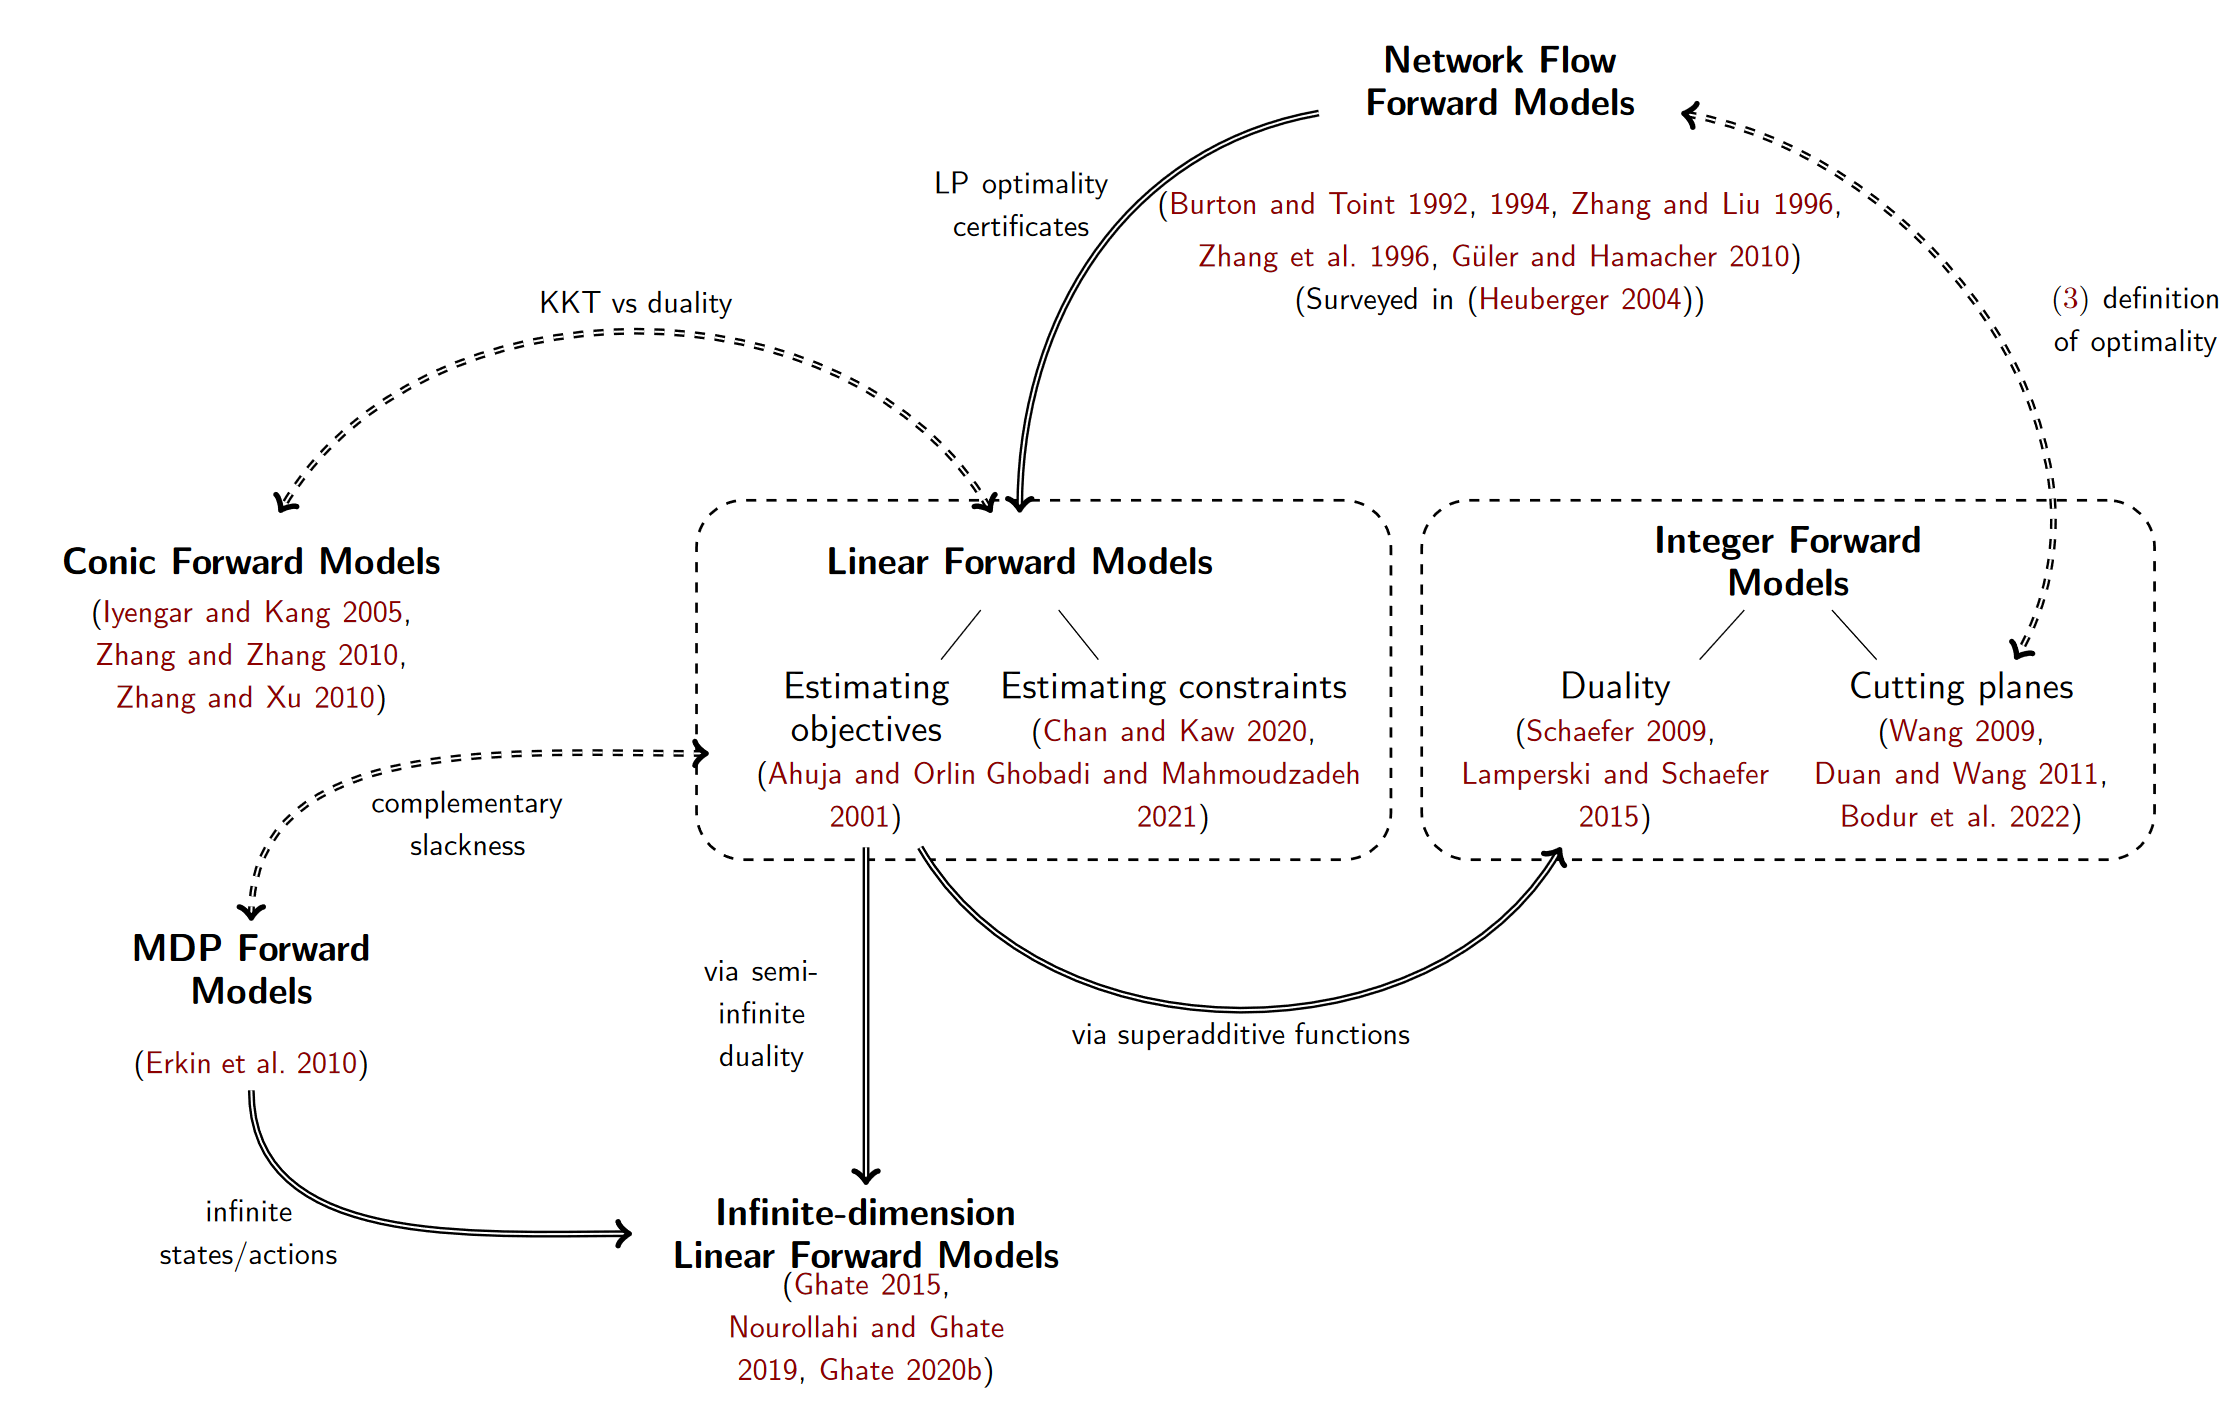
\includegraphics[width=\textwidth]{res/img/classical-io-roadmap}
    \caption{Roadmap of Classical IO from \cite{chanInverseOptimizationTheory2022}. Bold arrows denote extensions and
generalizations and dashed arrows denote conceptual similarities.}
    \label{fig:litrev:io-roadmap}
\end{figure}

\cite{chanInverseOptimizationTheory2022} survey the current state of the art in IO. They provide a taxonomy of IO problems by splitting them along three axes: forward model structure, parameter type, and model-data fit. The structure of the forward model (e.g. linear, mixed-integer, sequential, or conic) determines which kind of IO techniques can be used, and which parameters can be recovered. Parameter type refers to which problem parameters need to be recovered. This can be whether the objective parameters, the constraint parameters, or both are unknown. The authors of the survey split the field of IO into classical and data-driven IO, and call this split model-data fit. In the classical setting, every decision in the set of solutions is assumed to be optimal. In the data-driven setting, decisions contain some amount of noise and may not be optimal or even feasible. The taxonomy of classical IO is illustrated in Figure \ref{fig:litrev:io-roadmap}, taken from the survey. Data-driven IO is orthogonal to classical IO: the same techniques can be used, but instead of enforcing solution feasibility in the constraints of the inverse model, deviation from feasibility is penalized using an additional loss function in the objective.

Most IO literature focuses on the recovery of parameters in the objective function. However, in the case of ND, the unknown demand parameters appear in the constraints. \cite{bodurInverseMixedInteger2021} proposes an IO method for mixed-integer LPs, but is limited to the recovery of objective parameters. Methods for recovering the constraint parameters of integer or mixed-integer forward models do not exist as of yet. \cite{chanInverseOptimizationRecovery2020} and \cite{ghobadiInferringLinearFeasible2021} focus on recovering the constraint parameters of a LP. Both methods assume a linear forward problem with the following structure:
\begin{mini}
    {\bm{x}}
    {\bm{c}^\top \bm{x}}
    {(\text{Forward Problem})\label{eq:litrev:forward-problem}}
    {\qquad}
    \addConstraint{\bm{A}\bm{x}}{\geq \bm{b}}{}
    \addConstraint{\bm{x}}{\in \mathbb{R}^n}{}
\end{mini}
\cite{chanInverseOptimizationRecovery2020} assume the $\bm{c}$ and $\bm{b}$ vectors are known, and show a method for recovering the parameters in $\bm{A}$. \cite{ghobadiInferringLinearFeasible2021} consider the more general problem of recovering all the constraint parameters $\bm{A}$ and $\bm{b}$. In both papers, the resulting IO models contain bilinear terms in the constraints and must use observations about the forward problem structure in order to reduce the inverse model to a computationally tractable version. For example, \cite{ghobadiInferringLinearFeasible2021} observe that, given the optimal solution $\bm{x}^*$, $\bm{c}^\top \bm{x} \geq \bm{c}^\top \bm{x}^*$ is an implicit constraint of the forward problem. This observation allows them to formulate the following inverse model without the implicit constraints: 

\begin{minie}
    {\bm{A}, \bm{b}}
    {\mathcal{F}(\bm{A}, \bm{b}, \mathcal{D})}
    {(\text{eMIO}) \label{eq:litrev:inverse-ghobadi}}
    {\qquad}
  \addConstraint{\bm{a}^\top_k \bar{\bm{x}}^l}{\geq \bm{b}, \quad}{\forall\, k, l}
  \addConstraint{\lVert \bm{a}_k\rVert}{= 1, \quad}{\forall\, k}
  \addConstraint{\bm{A}}{\in \mathcal{A}_{\text{valid}}}{}
  \addConstraint{\bm{b}}{\in \mathcal{B}_{\text{valid}}}{}
\end{minie}
This models defines parameters $\bm{A}$ and $\bm{b}$, from their respective domains $\mathcal{A}_{\text{valid}}$ and $\mathcal{B}_{\text{valid}}$, which ensure all solutions $\{\bar{\bm{x}}\}_l$ are feasible. The choice of parameters $\bm{A}$ and $\bm{b}$ minimizes the cost function on the constraint parameters $\mathcal{F}(\bm{A}, \bm{b}, \mathcal{D})$. Various cost functions are possible to achieve desired properties of the recovered feasible region.

All of the inverse models discussed above have a key limitation for ILO pipelines: they do not yield a trained prediction model which can generalize to new instances of the demand prediction problem. For every new instance of the MCFND, the IO model would have to be re-run, using the new optimal solution to recover the demands. This cannot work in practical cases, since the actual demand and thus the actual optimal network is not known at the time of planning. This raises the following question: is there a way to train a demand prediction model using techniques from IO? 

A few months after the start of this thesis, \cite{sunMaximumOptimalityMargin2023} is published. They are the first to perform DFL with IO for linear prediction models and linear forward optimization models. They consider a CSO problem in which the objective parameters of the optimization are predicted using a linear regression model on the contextual information. The authors embed the prediction model inside of the forward optimization model, replacing the objective parameters with their respective linear regression prediction, i.e. $\bm{c}$ is replaced with $\hat{\bm{c}} := \bm{\Theta} \bm{\phi}$. The IO model recovers the linear regression weights $\bm{\Theta}$ that minimize task loss, given a training dataset of contextual features and corresponding optimal solutions $(\bm{\phi}, \bm{x}^*)$. To achieve this, the authors first define the optimal basis of an LP:
\begin{defin}[Optimal basis, \cite{sunMaximumOptimalityMargin2023}, p. 4]
Let $\bm{x}^* := (z_1^*, \ldots, z_n^*)$ be the optimal solution to the linear problem $\mathrm{LP}(c, A, b)$, with a cost vector $\bm{c} \in \mathbb{R}^n$, and $m$ constraints defined by $\bm{A} \in \mathbb{R}^{m\times n}$ and $\bm{b} \in \mathbb{R}^m$. The optimal basis $\mathcal{B}^*$ and its complement $\mathcal{N}^*$ is defined as follows:
$$\mathcal{B}^* := \{i : x^*_i > 0\}, \quad \mathcal{N}^* := \{i : x^*_i \leq 0\}$$
For a set $\mathcal{B} \subset [n]$, $A_{\mathcal{B}}$ denotes the submatrix of $A$ with columns indices corresponding to $\mathcal{B}$, and $c_\mathcal{B}$ denotes the subvector with corresponding dimensions.
\end{defin}
The authors use a property of the optimal basis of an LP which states, with minimal assumptions on the structure of the LP, that:
\begin{lemma}[Lemma 1 of \cite{sunMaximumOptimalityMargin2023}]
    \label{lemma:litrev:optimality}
    Let $\mathcal{B} \subset [n]$ be a feasible basis of $\mathrm{LP}(c, A, b)$, i.e. $A^{-1}_{\mathcal{B}}b \geq 0$ and let $\mathcal{N} = [n] \setminus \mathcal{B}$ be its complement. Then, if LP is non-degenerate, the following relation holds:
    $$c^\top_\mathcal{N} - c^\top_\mathcal{B} A^{-1}_\mathcal{B}A_\mathcal{N} \geq 0 \quad\Leftrightarrow\quad \mathcal{B} = \mathcal{B}^*$$ 
\end{lemma}
Using this property, the authors formulate their IO model for $\mathrm{LP}(c, A, b)$, given training data $\mathcal{D}_\mathrm{train} = \{(\phib_l, x^*_l, A_l, b_l, \mathcal{B}^*_l, \mathcal{N}^*_l)\}_{l=1}^L$:

\begin{argminie}[1]
    {\Theta}
    {\dfrac{\lambda}{2}\lVert \Theta \rVert^2_2 + \dfrac{1}{L} \sum_{l=1}^L \lVert s_l \rVert_1 \label{eq:litrev:mom-objective}}
    {(Maximum-Optimality-Margin) \label{eq:litrev:mom}}
    {\hat{\Theta} :=}
    \addConstraint{\hat{c}_l}{= \Theta\phib_l, \quad \label{eq:litrev:mom-prediction}}{\forall l=1, \ldots, L }
    \addConstraint{\hat{c}^\top_{l,\mathcal{N}^*_l} - \hat{c}^\top_{l,\mathcal{B}^*_l} A^{-1}_{l, \mathcal{B}^*_l} A_{l, \mathcal{B}^*_l}}{\geq \mathbbm{1}_{|\mathcal{N}^*_l|} - s_l, \quad \label{eq:litrev:mom-slackness}}{\forall l=1, \ldots, L}
\end{argminie}
Constraints (\ref{eq:litrev:mom-prediction}) encode the linear prediction of the cost vector $\hat{c}_l$ into the model, using weights $\Theta$ and contextual information $\phib_l$. The left hand side of constraint (\ref{eq:litrev:mom-slackness}) represents the optimality condition from Lemma \ref{lemma:litrev:optimality}, and the right hand size captures the violation, or \textit{slackness}, of the optimality constraint for that prediction, encoded in the variable $s_l$. The objective (\ref{eq:litrev:mom-objective}) regularizes the weights $\Theta$ and minimizes the mean absolute deviation from the optimality conditions.

This method yields a trained linear prediction model $f_{\bm{\Theta}}$ with weights $\hat{\Theta}$ which predicts costs $\bm{c}$ for contextual features $\bm{\phi}$ without knowing their corresponding optimal optimization solution $\bm{x}^*$. This model produces predictions $\hat{c}$ that minimizes deviation from optimality in the downstream optimization problem, which means this model minimizes task loss. However, this is limited to predicting the objective parameters of linear optimization models and cannot predict constraint parameters of mixed-integer models.

IO offers advanced techniques for recovering parameters of optimization problems given a set of solutions. It supports multiple types of optimization models, can recover parameters in the objective and in the constraints, and can handle noise and uncertainty in the data. Generally, it lacks the ability to generalize to new instances of the same problem without re-solving the IO. However, new research offers a promising direction in which a linear prediction model is trained to minimize task loss using IO. 

\section{Discussion} \label{sec:litrev:discussion}

ND is a well researched subject in operations research. Many works focus on finding more efficient ways to solve large instances of the MCFND. The complexity and combinatorial nature of ND problems means that stochastic formulations are often not computationally tractable. Thus, most of the research concentrates on the deterministic version of ND, with the parameter prediction steps left separate. 

The idea of DFL, integrating the prediction and optimization steps in a data-decisions pipeline, is relatively recent. Research in this field originated in the ML and operations research community. The key technique involves training a prediction model using gradient descent on the downstream task loss, or \textit{regret}. This implies differentiating through the $\arg\min$ of the optimization problem, which can be done using implicit differentiation, differentiable surrogate loss functions, or differentiable surrogate models. Current works focus on predicting cost function coefficients, and are mostly restricted to problems with continuous variables, with the exception of \textit{CombOptNet} from \cite{paulusCombOptNetFitRight2022}.

IO is a more developed field than DFL. Given solutions to a forward optimization model with unknown parameters, an IO model recovers parameters that make the decisions optimal. Several techniques to recover constraint parameters of LPs exist, though none for MILPs yet, and IO can handle uncertainty in the solution dataset using data-driven IO. However, IO does not yield a prediction model that can be used on new instances of the problem, which limits its use in the ND pipeline. Recent research by \cite{sunMaximumOptimalityMargin2023} shows how to use IO to train a linear prediction model that predicts objective parameters that minimize task loss.

In this chapter, we have reviewed the three related areas of ND, DFL, and IO. Our setting is often formulated as the stochastic MCFND problem. There are several studies on stochastic ND, but real-world applications use the deterministic formulation of the MCFND. Solving an ND problem as a stochastic program turns out to be too computationally expensive, despite the improvements in decision quality. Therefore, real-world applications use point predictions for the parameters of the optimization model. This led us to investigate DFL and IO to find how to improve the quality of the point predictions. DFL could be used with stochastic programming, e.g. decision-focused density estimation is possible for CSO problems, as shown in \cite{sadanaSurveyContextualOptimization2023}, but research on this topic is still limited. For this reason, and due to the computational limitations of stochastic ND, we restrict this work to DFL and IO making point predictions. 
Most of the research in DFL and IO to date focuses on linear optimization programs, with continuous variables and uncertainty only in the objective. However, our use case involves complex MILPs with uncertain parameters in the constraints. Nevertheless, we have identified key ideas that could help our task of integrating the prediction and optimization steps of a ND problem with uncertain demands. All of them rely on a good definition of regret, the cost of the downstream optimization problem. Regret is well-defined when only the objective parameters are uncertain, and many systems offers ways to minimize regret in this case. Some systems offer interesting ways to recover uncertain constraint parameters, such as \textit{CombOptNet}, but use simpler, differentiable, loss functions and not regret. \textit{CombOptNet} also suffers from computational performance issues that may be addressed by other techniques from the literature. By making connections to the separate field of IO, we could improve DFL methods. Recent work by \cite{sunMaximumOptimalityMargin2023} on using IO to train a prediction model that minimizes regret for uncertain costs could be combined with constraint recovery techniques from \cite{chanInverseOptimizationRecovery2020} or \cite{ghobadiInferringLinearFeasible2021} to create an alternative method of training DFL pipelines.
